
\begin{figure}
\centering
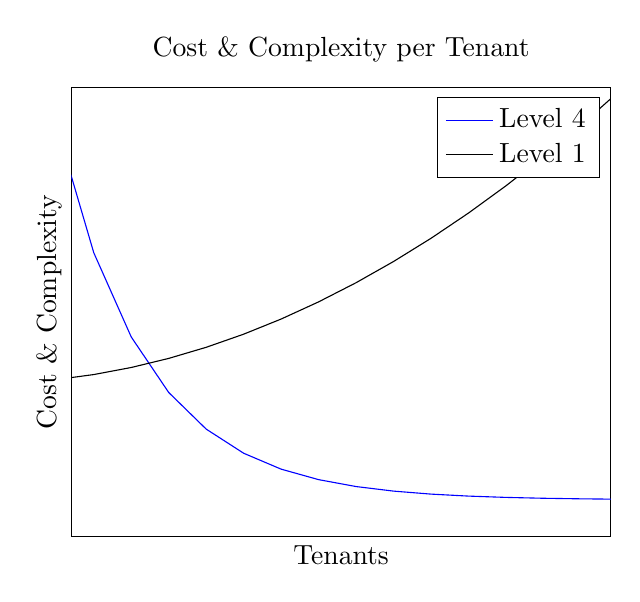
\begin{tikzpicture}
\begin{axis}[
    title={Cost \& Complexity per Tenant},
    ymajorticks=false,
    xmajorticks=false,
    xlabel={Tenants},
    ylabel={Cost \& Complexity},
    ymajorgrids=false,
    xmin=-4, xmax=2,
    grid style=dashed,
]
 
\addplot[color=blue]{exp(-x)};
	
	\addplot[color=black] {0.5(x+5)^2 + 20	};
	
\legend{Level 4, Level 1}
\end{axis}
\end{tikzpicture}

\caption{Implementation complexity per tenant}
\label{fig:imp_complexity}
\end{figure}




